%!TEX root =  ../Report.tex
% %Here are some subsections so that they will appear on the contents
\subsection{Classifiers}

%Classification on the combined set of features was conducted against three classifier models, Random Forest (RF), XGBoost and K-Nearest Neighbour (KNN).

\subsubsection{Random Forest (RF)}
\label{sec:RF}

Initial modelling began using stock parameters without changing or adding any values. Due to the nature of training time, we did not utilise GridSearchCV for hyperparameter tuning. Instead, we used a series of settings and parameters to get an optimal model. Each model was trained on the entire training dataset to gauge initial performance, before using 10-fold Stratified Cross Validation and evaluating finally on the test set. Table \ref{tab:rf-params} shows the parameters considered during the creation and optimisation of the models. For the context of the device, the majority of Random Forest models were trained using the VM.

\begin{table}[h]
\centering
\caption{Parameters for Random Forest Classifier}
\label{tab:rf-params}
\begin{tabular}{|l|l|l|}
\hline
\textbf{Parameter} & \textbf{Description} \\ \hline
n\_estimators & The number of trees in the forest\\
criterion & Function to measure the quality of a split.\\
max\_depth & Maximum depth of the tree. \\
min\_samples\_split & Minimum samples required to split an internal node. \\ 
min\_samples\_leaf & Minimum samples required to be at a leaf node. \\
max\_features & Maximum features to consider when splitting. \\
bootstrap & To bootstrap samples when constructing trees \\
class\_weight & Weights associated with classes \\
random\_state & The random seed.\\ \hline
\end{tabular}
\end{table}

% \begin{table}[h]
% \centering
% \caption{RF Model Metrics}
% \label{tab:rf-metrics}
% \begin{tabular}{|l|l|l|l|l|l|l|}
% \hline
% \textbf{Model} & \textbf{Data Subset} & \textbf{Accuracy} & \textbf{Precision} & \textbf{Recall} & \textbf{F1} & \textbf{Time} \\ \hline
% Base & 80\% & 0.997 & 0.955 & 0.882 & 0.916 & 00:02:34:59 \\ \hline
% Base & 100\% & 0.997 & 0.997 & 0.997 & 0.997 & 00:00:30:60 \\ \hline
% \end{tabular}
% \end{table}

%\begin{table}[h]
%\centering
%\caption{RF Evaluation Set Metrics}
%\label{tab:rf-metrics}
%\begin{tabular}{|l|l|l|l|l|l|}
%\hline
%\textbf{Model} & \textbf{Data Size} & \textbf{Accuracy} & \textbf{Precision} & \textbf{Recall} & \textbf{F1}  \\ \hline
%Stock & 80\% & 0.997 & 0.955 & 0.882 & 0.916  \\ \hline
%Stock & 100\% & 0.997 & 0.997 & 0.997 & 0.997 \\ \hline
%\end{tabular}
%\end{table}

\begin{table}[h]
\centering
\caption{RF S-CV Mean Metrics}
\label{tab:rf-scv-metrics}
\begin{tabular}{|l|l|l|l|l|l|l|}
\hline
\textbf{Model} & \textbf{Size} & \textbf{AUC} & \textbf{F1} & \textbf{Precision} & \textbf{Recall} & \textbf{Accuracy}  \\ \hline
Stock & 100\% & 99.99 & 99.66 & 99.66 & 99.67 & 99.67 \\ \hline
Model 1 & 100\% & 99.99 & 99.66 & 99.66 & 99.67 & 99.67 \\ \hline
Model 2 & 100\% & 99.95 & 95.23 & 98.50 & 92.96 & 92.96 \\ \hline
Model 3 & 100\% & 99.87 & 91.53 & 98.42 & 86.65 & 86.65 \\ \hline
\end{tabular}
\end{table}


\begin{table}[h]
\centering
\caption{RF Evaluation Set Metrics}
\label{tab:rf-eval-metrics}
\begin{tabular}{|l|l|l|l|l|l|l|}
\hline
\textbf{Model} & \textbf{Size} & \textbf{AUC} & \textbf{F1} & \textbf{Precision} & \textbf{Recall} & \textbf{Accuracy}  \\ \hline
Stock & 100\% & 99.99 & 99.66 & 99.66 & 99.67 & 99.67 \\ \hline
Model 1 & 100\% & 99.99 & 99.66 & 99.66 & 99.67 & 99.67 \\ \hline
Model 2 & 100\% & 99.95 & 95.23 & 98.50 & 92.96 & 92.96 \\ \hline
\end{tabular}
\end{table}


\begin{table}[h]
\centering
\caption{RF Model Parameters}
\label{tab:rf-parameters}
\begin{tabular}{llllll}
\hline
Parameter & Model 1 & Model 2 \\ \hline
n\_estimators: & 100 & 200 \\
max\_depth: & 10 & 15  \\
min\_samples\_leaf: & 2 & 1  \\
min\_samples\_split: & 3 & 2  \\
random\_state: & 1234 & 1234 \\
class\_weight: & None & balanced \\ \hline
\end{tabular}
\end{table}

%\paragraph{Confusion Matrix}
%
%\begin{figure}[H]
%    \centering
%    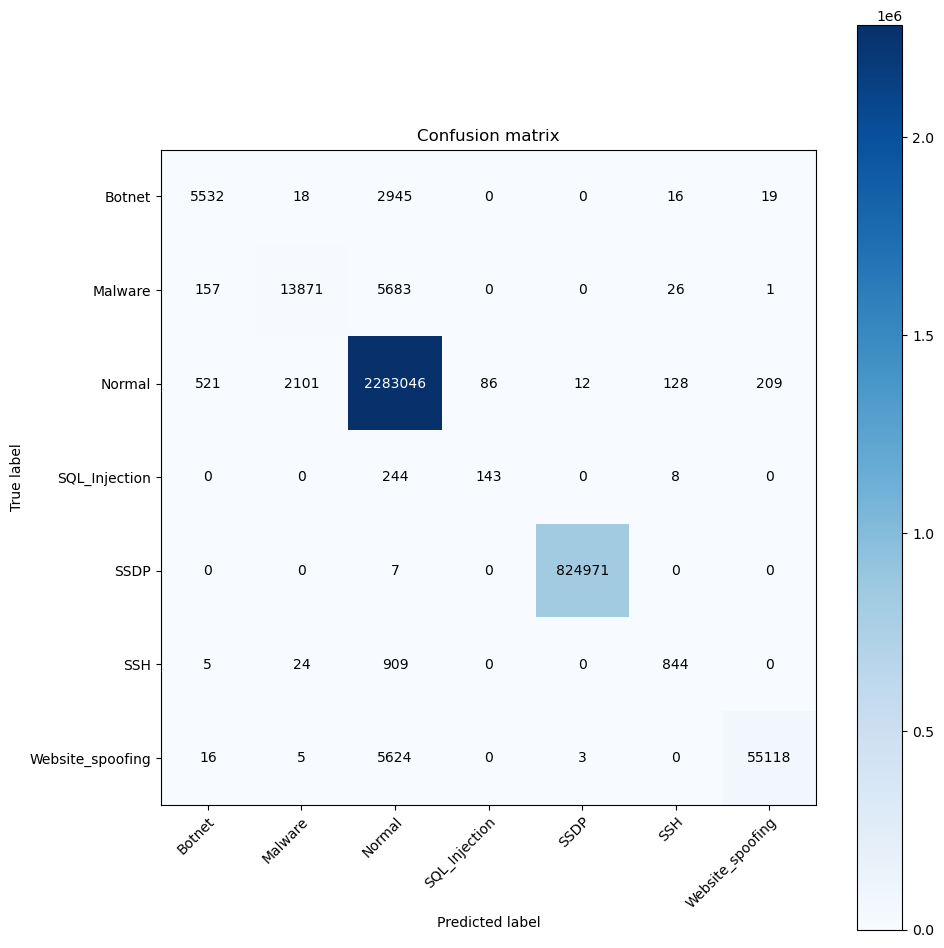
\includegraphics[width=0.85\textwidth]{Appendices/NN Confusion Matrix 3-04-23.png}
%    \caption{RF Confusion Matrix}
%    \label{fig:rf_confusion_matrix}
%\end{figure}
